\section*{Neural Networks}

$F(x)=W^{L}\phi^{L-1}(W^{L-1}...(\phi^{1}(W^{1}x)...))$

$\textbf{ReLU: } \max (0,z), \; \textbf{Tanh: } \frac{\exp(z) - \exp(-z)}{\exp(z) + \exp(-z)}$ \\[-3pt]
$\textbf{Sigmoid: } \varphi(z) = \frac{1}{1 + \exp(-z)}, \varphi' = (1 - \varphi) \varphi$


\textbf{Universal Approximation Theorem}: We can approximate any arbitrary smooth target function, with 1+ layer with sufficient width.

\subsection*{Forward Propagation}

Input: $v^{(0)} = [x; 1]$ \quad Output: $f = W^{(L)} v^{(L-1)}$
Hidden: $z^{(l)} = W^{(l)} v^{(l-1)}, v^{(l)} = [\varphi(z^{(l)}); 1]$


\subsection*{Backpropagation}

Non-convex optimization problem: \\[-10pt]

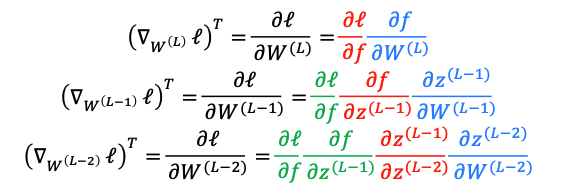
\includegraphics[width=\columnwidth]{backpropagation.png} \\[-15pt]

Only compute \color{Red} \textbf{the gradient}\color{Black}. Rand. init. weights by distr. assumption for $\varphi$. ( $2 / n_{in}$ for ReLu and $1/n_{in}$ or $ 1/ (n_{in} + n_{out})$ for Tanh)

\subsection*{Overfitting}
\textbf{Regularization}; \textbf{Early Stopping}; \textbf{Dropout}: ignore hidden units with prob. $p$, after training use all units and scale weights by $p$; \textbf{Batch Normalization}: normalize the input data (mean 0, variance 1) in each layer

\subsection*{CNN \quad \color{Black}$\varphi(W * v^{(l)})$}

The output dimension when applying $m$ different $f \times f$ filters to an $n \times n$ image with padding $p$ and stride $s$ is: $l = \frac{n + 2p - f}{s} + 1$

For each channel there is a separate filter.